\chapter{Lecture} %%% 31
\markboth{\thechapter. Lecture}{\thechapter. Lecture}

We\pageoriginale want to prove directly the reciprocity formula
$$
\displaylines{
  s(h, k)+ s(k, h)=- \frac{1}{4} + \frac{1}{12} \left( \frac{h}{k} +
  \frac{k}{h} + \frac{1}{hk}\right)\cr
  \text{with} \hfill s(h, k)= \sum^k_{\mu=1} \frac{\mu}{k} \left(
  \left( \frac{h\mu}{k}\right) \right)\phantom{WWW}\hfill }
$$

The reciprocity formula is equivalent to proving that
$$
12h \sum^{k-1}_{\mu=1} \mu \left[ \frac{h \mu}{k}\right]+ 12k
\sum^{h-1}_{\nu=1} \nu \left[\frac{k \nu}{h} \right] = (h-1)(k-1)(8hk-h-k-1)
$$

We made a little digression and spoke of similar sums which occur in
lattice-point summations:
$$
\sum^{k-1}_{\mu=1} \left[ \frac{h \mu}{k}\right]+ 
\sum^{h-1}_{\nu=1} \left[\frac{h \nu}{h} \right]= (h-1)(k-1)
$$

If we use a rectangle of sides $\frac{h}{2}, \frac{k}{2}, (h, k
~\text{odd})$ we obtain 
$$
\sum^{\frac{k-1}{2}}_{\mu=1} \left[ \frac{h \mu}{k}\right]+  
\sum^{\frac{h-1}{2}}_{\nu=1} \left[\frac{h \nu}{h} \right] = 
\frac{1}{4} (h-1)(k-1).
$$

This is made use of the theory of quadratic residues.

The summands in our case are `quadratic' in $\mu$ and $\nu$.
\begin{figure}[H]
  \centering{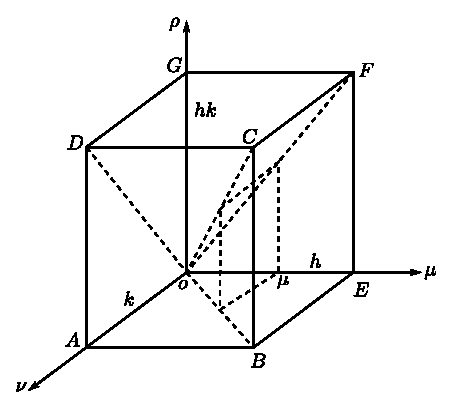
\includegraphics{vol2-figures/fig2.39.eps}}
\end{figure}

Consider\pageoriginale the rectangular parallelopiped with three concurrent edges
along the axes of $\mu$, $\nu$ and $\rho$, the lengths of these edges
being $h$, $k$, $hk$ respectively. Dissect the parallelopiped into
three pyramids having a common apex at the origin and having for bases
the three rectangular faces which do not pass through the origin,
viz. $ABCD$, $BCFE$ and $CDGF$. We now compute the number of lattice
points in each pyramid. Take for example the pyramid
$O(BEFC)$. Consider a section parallel to the $(\rho, \nu)$-plane at a
distance $\mu$ along the $\mu$-axis. The lattice points lie in such
sheets. The edges of this section are $h\mu$ and $\mu
\frac{h}{k}$. The number of lattice points on this sheet (including
possibly those on the edges) is $h \mu \left[\frac{\mu h}{k}
  \right]$. So for the whole pyramid the number
$=\sum\limits^{k-1}_{\mu=1} h \mu \left[ \frac{ \mu h}{k}\right]$. For
the pyramid $O(ABCD)$, the one facing us, the number is
$\sum\limits^{h-1}_{\nu=1} k \nu \left[ \frac{\nu k}{h}\right]$ 

Of\pageoriginale course are some points on the common edge. Finally
there is a pyramid of exceptional sort which lies upside
down. Consider a section at a height $h$ parallel to the $(\mu, \nu)$
plane the number of lattice points on and inside this pyramid is seen
to be 
$$
\sum_{\rho=1}^{hk-1} \left[ \frac{\rho}{h} \right] \left[\frac{\rho}{k}
  \right]. 
$$

So altogether we have
$$
\sum^{k-1}_{\mu=1} h \mu \left[ \frac{\mu h}{k}\right]+
\sum^{h-1}_{\nu=1} k \nu \left[ \frac{\nu k}{k}\right]+
\sum^{hk-1}_{\rho=1} \left[\frac{\rho}{h} \right] \left[\frac{\rho}{k}
  \right] 
$$
points, including some points which have been counted twice over. But
the number of lattice points \textit{inside}: the parallelopiped is
equal to $(h-1)(k-1)(hk-1)$. Hence making a correction for the lattice
points on the cleaving surfaces through the edges $CF$ and $CD$ which
have been counted twice (the surface along $BC$ has no points on it
because $(h, k)=1$), we have
\begin{align*}
  \sum^{k-1}_{\mu=1} h \mu \left[\frac{\mu h}{k} \right] & +
  \sum^{h-1}_{\nu=1} k \nu \left[\frac{\nu k}{h} \right] +
  \sum^{hk-1}_{\rho=1} \left[\frac{\rho}{k}
    \right]\left[\frac{\rho}{h} \right] \\
   & =(h-1)(k-1)(hk-1)+ (h-1)(k-1)\\
   & = hk (h-1)(k-1)
\end{align*}

Now write
\begin{align*}
  S & = \sum^{hk-1}_{\rho=1} \left[\frac{\rho}{h}
    \right]\left[\frac{\rho}{k} \right]\\
  \left[\frac{\rho}{h} \right] & = \frac{\rho}{h} - \frac{1}{2} -
  \left( \left( \frac{\rho}{h}\right) \right), ~\text{if}~ h\nmid \rho;
  \frac{\rho}{h} - \left(\left( \frac{\rho}{h}\right)\right),
  ~\text{if}~ h\nmid \rho.
\end{align*}

So\pageoriginale
$$
S= \sum^{hk-1}_{\rho=1}\left\{ \frac{\rho}{h} - \frac{1}{2} - \left(
\left( \frac{\rho}{h}\right)\right)\right\} \left\{ \frac{\rho}{2} -
\frac{1}{2}-\left( \left( \frac{\rho}{k}\right)\right)\right\}
$$

With some correction. Indeed $h\mid \rho$, $k\mid\rho$ do not happen
together: Let $\rho = h \sigma$, $\rho = k \tau$. In the first
case. i.e., $h\mid \rho$, we have to correct the above by an amount
$$
\sum^{k-1}_{\sigma=1} \frac{1}{2} \left\{ \frac{h \sigma}{k} -
\frac{1}{2} - \left( \left(\frac{h \sigma}{k}\right)\right)\right\},
$$
and in the second case, $k\mid \rho$, by
$$
\sum^{h-1}_{\tau=1} \frac{1}{2} \left\{\frac{k \tau}{h}- \frac{1}{2} 
- \left(\left( \frac{k \tau}{h}\right)\right)\right\}
$$

So
\begin{multline*}
  S= \sum^{hk-1}_{\rho=1} \left\{ \frac{\rho}{h} - \frac{1}{2}\right\}
  \left\{ \frac{\rho}{k} - \frac{1}{2}\right\} - \sum^{hk}_{\rho=1}
  \left( \left(\frac{\rho}{h}\right)\right)\left(\frac{\rho}{k} -
  \frac{1}{2}  \right)- \sum^{hk}_{\rho=1} \left(
  \left(\frac{\rho}{k}\right)\right) \left( \frac{\rho}{h} -
  \frac{1}{2}\right)\\
  + \sum^{hk}_{\rho=1} \left( \left(\frac{\rho}{h}\right)\right)
  \left( \left(\frac{\rho}{k}\right)\right)+ \frac{1}{2}
  \sum^{k-1}_{\sigma=1} \left\{ \frac{h \sigma}{k} -
  \frac{1}{2}\right\}+ \frac{1}{2} \sum^{h-1}_{\tau=1} \frac{1}{2}
  \left\{ \frac{k \tau}{h} - \frac{1}{2}\right\}   
\end{multline*}

Since $\sum\limits_{\mu \mod k}\left(
\left(\frac{\mu}{k}\right)\right)=0$, \quad this becomes 
\begin{multline*}
  S = \sum^{hk-1}_{\rho=1} \left\{ \frac{\rho^2}{hk} - \frac{1}{2}
  \left( \frac{\rho}{h} + \frac{\rho}{k}\right)+ \frac{1}{4}\right\}-
  \frac{1}{4} \sum^{hk}_{\rho=1} \rho \left(
  \left(\frac{\rho}{k}\right)\right)- \frac{1}{h} \sum^{hk}_{\rho=1}
  \rho \left( \left(\frac{\rho}{k}\right)\right)\\
  +\sum^{hk}_{\rho=1} \left( \left(\frac{\rho}{h}\right)\right)
  \left( \left(\frac{\rho}{k}\right)\right)+ \frac{1}{2} \left(
  \frac{h(k-1)}{2} - \frac{k-1}{2}\right) + \frac{1}{2} \left(
  \frac{k(h-1)}{2} - \frac{h-1}{2}\right)  
\end{multline*}\pageoriginale
we use the periodicity in the non-elementary pieces; so write
\begin{align*}
  \rho & = hr+s; r=0,1, \ldots, k-1; s=1, \ldots, h.\\
  \sum^{hk}_{\rho=1} \rho \left( \left(\frac{\rho}{h}\right)\right) &
  = \sum^{k-1}_{r=0} \sum^{h}_{s=1} (hr+s)
  \left(\left(\frac{hr+s}{h}\right)\right)\\
  & = \sum^{k-1}_{r=0} \sum^{h}_{s=1} hr \left(
  \left(\frac{s}{h}\right)\right)+ \sum^{k-1}_{r=0}\sum^h_{s=1} s
  \left(\left(\frac{s}{h}\right)\right)    \\
  & = k \sum^h_{s=1} s \left( \left(\frac{s}{h}\right)\right) 
\end{align*}
(since the first sum is zero, as we see by summing over $s$ first)
\begin{align*}
  & = k \sum^{h-1}_{s=1} s\left( \frac{s}{h} - \frac{1}{2}\right)\\
  & = k \left\{\frac{(h-1)(2h-1)}{6} - \frac{1}{4} h (h-1) \right\}\\
  & = \frac{k(h-1)(h-2)}{12}
\end{align*}

Similarly\pageoriginale
$$
\sum^{hk}_{\rho=1}\rho \left( \left(\frac{\rho}{k}\right)\right)=
\frac{h(k-1)(k-2)}{12}  
$$
next, consider 
$$
\sum^{ik}_{\rho=1} \left( \left(\frac{\rho}{h}\right)\right) \left(
\left(\frac{\rho}{k}\right)\right)  
$$

Write $\rho= h \alpha + k \beta$; when $\alpha$, $\beta$ run through
complete systems of residues modulo $h$, $k$ respectively, $h \alpha +
k \beta$ runs through a complete system modulo $hk$, by the Chinese
remainder theorem. Then
\begin{align*}
  \sum^{hk}_{\rho=1} \left(\left(\frac{\rho}{h}\right)\right)
  \left(\left(\frac{\rho}{k}\right)\right)   & = \sum_{\alpha \mod k}~
  \sum_{\beta \mod h} \left(\left(\frac{h \alpha + k
    \beta}{h}\right)\right)\left(\left(\frac{h \alpha + k
    \beta}{k}\right)\right)\\
  & = \sum_{\alpha \mod k}~ \sum_{\beta \mod h}
  \left(\left(\frac{k \beta}{h}\right)\right)
  \left(\left(\frac{h \alpha}{k}\right)\right)\\
  & = \sum_{\alpha \mod k} \left(\left(\frac{h
    \alpha}{k}\right)\right) \sum_{\beta \mod h}
  \left(\left(\frac{k \beta}{h}\right)\right)\\
  & = 0
\end{align*}
since each sum is separately zero. Hence
\begin{align*}
  S & = \frac{1}{6} (hk-1)(2h k-1)- \frac{1}{4} (hk-1)(k+h)+ \frac{1}{4}
  (hk-1)\\ 
    & \qquad - \frac{1}{12} (h-1)(h-2)- \frac{1}{12} (k-1)(k-2)+
  \frac{1}{2} (k-1)(h-1)\\
  & = \frac{1}{12} (hk-1) (4hk-3 h-3 k+1)- \frac{1}{12} (h-1)(h-2)\\
  & \hspace{3cm}- \frac{1}{12} (k-1)(k-2) + \frac{1}{2} (k-1) (h-1)\\
  & = \frac{1}{12} (h-1)(k-1)(4 hk + h + k+1)
\end{align*}

Thus\pageoriginale
\begin{align*}
  h \sum^{k-1}_{\mu=1} \mu \left[ \frac{h \mu}{k}\right] & + k
  \sum^{h-1}_{\nu=1} \nu \left[\frac{k \nu}{h} \right]+ \frac{1}{12}
  (h-1)(k-1)(4hk+h+k+1)\\
  & = (h-1)(k-1) hk\\
  \therefore \quad 12h \sum^{k-1}_{\mu=1} \mu \left[ \frac{h
      \mu}{k}\right] & + 12 k \sum^{h-1}_{\nu=1} \nu \left[ \frac{k
      \mu}{h}\right]\\
  & = (h-1) (k-1)(8hk-h-k-1)
\end{align*}

We make some elementary remarks about quadratic residues. The
reciprocity formula gives, on multiplication by $12h^2 k$.
$$
12h^2 k s(h, k)+ 12 h^2 k s(k, h)= =- 3h^2k + h^3 + k^2 h
$$

Look\pageoriginale at the denominator of $s(h, k)$. At worst it can
have for factors 2 and $k^2$. So $2k^2 s(h, k)$ is integral. $2 h^2
s(k, h)$ is also integral.
\begin{align*}
  12 h^2 k s(h, k) & \equiv h^3 + k^2 + h \pmod{3k}\\
  & \equiv h(h^2 + 1) \pmod{k},
\end{align*}
and since $h^2$ cannot help to make an integer of the left side,
$$
12 hk s(h, k)\equiv h^2 + 1 \pmod{k}.
$$

Sp $12k s(h, k)$ is an integer. The highest possible denominator for
$s(h, k)$ is $(2k^2, 12k)= 2k(k, 6)$. So the denominator which at
first glance could conceivably be as big as $2k^2$ is actually at most
only $2k (k, 6)$. This is achieved, for instance, in $s(1,3)=1/18$,
where $6(6,3)=18$. In fact $s(1,3)$ can be computed from the
reciprocity formula:
$$
s(1, 3)+ s(3, 1)=- \frac{1}{4} + \frac{1}{12} \left( \frac{1}{3} +
\frac{3}{1} + \frac{1}{3}\right) s(3, 1)=0
$$
since an integer is involved and so $s(1,3)= \frac{1}{18}$. In
general,
\begin{align*}
  s(1, k)& = - \frac{1}{4} + \frac{1}{12} \left( \frac{1}{k} +
  \frac{k}{1} + \frac{1}{k}\right)\\
  & = \frac{(k-1)(k-2)}{12k}
\end{align*}
$s(2, k)$ is also easily obtained. $k$ is odd; so we have
$$
s(2, k)+ s(1, 2)= - \frac{1}{4} + \frac{1}{12} \left(\frac{2}{k} +
\frac{k}{2} + \frac{1}{2k} \right)
$$
and\pageoriginale as $s(1, 2)=0$ (by direct computation), we get 
$$
s(2, k)= \frac{(k-1)(k-5)}{2 4k}
$$

Let us calculate $s(5, 27)$.
\begin{align*}
  s(5, 27)+ s(27, 5)& = - \frac{1}{4} + \frac{1^2 + 5^2 + 27^2}{12
    \times 5 \times 27}\\
  s(2, 5)+ s(5, 2) & = - \frac{1}{4} + \frac{1^2 + 2^2 + 5^2}{12
    \times 2 \times 5}\\
  s(5, 2) & = 0 = s(1, 2), \quad \text{and on sub traction},\\
  s(5, 27) & = 35/(6 \times 27); \quad \text{and we know that}
\end{align*}
the denominator could be at most $2.27(27,6)= 6 \times 27$.
